\chapter{Modellezés}
A probléma négy lényeges részből áll, amelyeket többé-kevésbé külön lehet kezeni egymástól:
\begin{enumerate}
	\item Balun
	\item Differenciális vonal
	\item Antenna
	\item Földkitöltésben gerjesztett áramokat csökkentő mintázat
\end{enumerate}
\par Ezek fejlesztése több szempontból is párhuzamosan kellett, hogy történjen, mert sem a balun, sem az antenna nem valósítható meg széles paramétertartományban. Az egyik lényeges korlátozó paraméter a hullámimpedancia -- az antenna bemeneti impedanciáját a balun kimeneti impedanciájához kell illeszteni a kérdéses frekvenciatartományban (\SIrange{2405}{2485}{MHz}) és természetesen ehhez az impedanciához kell méretezni az antennát tápláló differenciális vonal hullámimpedanciáját, hogy ez se okozzon lényeges reflexiót.
\section{Differenciális vonal}
Mivel az antenna differenciális táplálású, érdemes differenciális tápvonallal gerjeszteni. Az antenna által lefedett terület alatt nem célszerű földkitöltést használni az alsóbb rézrétegeken, mert ezek erősen lerontanák az antenna tulajdonságait. Így a tápláló differenciális vonalnak is olyannak kell lennie, hogy nincs alatta földkitöltés. Egy ilyen tápvonal a koplanár differenciális vonal (coplanar strip, CPS). A tápvonal keresztmetszete \aref{fig:cps}. ábrán látható.
\begin{figure}[h]
	\centering
	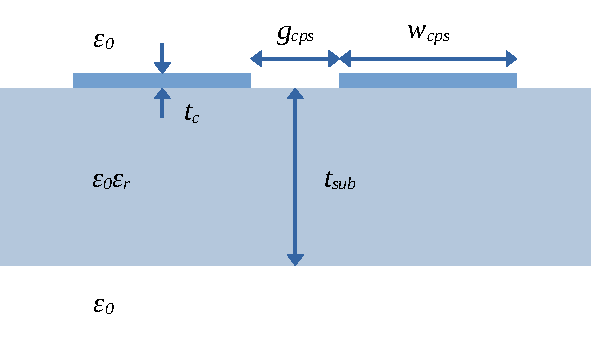
\includegraphics[width=0.6\textwidth]{kep/cps.pdf}
	\caption{Az antennát tápláló differenciális koplanár vonal (CPS) keresztmetszete.}
	\label{fig:cps}
\end{figure}
\par Sajnos az ilyen tápvonalakban nem lehetséges a TEM hullámterjedés, mivel a vezetők közötti elektromos erővonalak egy része a hordozó anyagában záródik, míg egy másik részük a levegőben, emiatt ugyanannak a haladó hullámnak egyes részei különböző sebességgel haladnak a vonalon, longitudinális térerősség-komponenseket hozva létre. Ez a jelenség pedig diszperzióhoz vezet és megbonyolítja a tápvonal hullámimpedanciájának definícióját is.
\par A CPS relatíve nehezen kezelhető volta miatt ritkábban használják, mint például a CPW tápvonalat. A CPS-t leíró közelítő formulák is kevésbé elterjedtek, nagyobb egyszerűsítésekkel adódnak és emiatt ez a tápvonal nem is szerepel az ismertebb impedanciakalkulátor programokban, mint például a KiCAD, vagy az AWR MWO programcsomagokhoz tartozó, vagy internetes kalkulátorokban. A tápvonal hullámimpedanciáját a CST ,,Waveguide Port'' funkcióját használva becsültem meg. Ilyen port használatakor a szimuláció során kiszámolódnak különböző módusok a porthoz (ami a CPS keresztmetszetéhez illeszkedik) és egy meghatározott alap módusra (differenciális, odd mode) adódó hullámimpedanciával számol tovább a program. Az így adódó értéket használtam fel, mint hullámimpedancia értéket.
\par Az említett nehézségek miatt ezt a pontatlanságot elfogadtam, ezzel együtt dolgoztam. Ezt a becslést az is alátámasztja, hogy egy hasonló felépítésű tápvonal, a slotline impedanciájával alulról becsülhető az azonos hézaggal és szubsztráttal elkészített CPS impedanciája. A slotline keresztmetszete a CPS-ével megegyező, azzal a kivétellel, hogy a két vezető oldalirányban sokkal nagyobb kiterjedésű, gyakorlatilag a teljes rendelkezésre álló felületet kitölti, végtelennek tekinthető. A nagyobb kiterjedésű vezetők közötti hosszegységre jutó kapacitás nagyobb, ezáltal a hullámimpedancia kisebb, mint a CPS esetében. Az összehasonlításhoz használt méretek és hullámimpedancia értékek \aref{tab:slotline-cps}. táblázatban láthatóak.
\begin{table}[h!]
	\centering
	\begin{tabular}{||c|c|c|c|c||c|c||}
	\hline
	$\varepsilon_r$ & $t_{sub}$ & $t_{c}$ & $g_{cps}$ & $w_{cps}$ & $Z_{c}$ & $Z_{slotline}$ \\ [0.5ex] 
	\hline\hline
	4,3 & \SI{1,55}{mm} & \SI{0,03}{mm} & \SI{0,274}{mm} & \SI{0,8}{mm} & \SI{100,19}{\ohm} & \SI{74,4}{\ohm}\\
	\hline
	\end{tabular}
	\caption{asd}
	\label{tab:slotline-cps}
\end{table}
Ennél a becslésnél a kétféle tápvonal közötti egyetlen különbség a 
\section{A nyomtatott balun transzformátor}
	A struktúrában a balun (balanced-unbalanced) transzformátor feladata a rádió kimenetétől érkező 50 Ohm-os, aszimmetrikus tápvonal és az antennát tápláló differenciális vonal egymáshoz illesztése minimális reflexióval. A rádió felől érkező tápvonalnak (és egyben a balun aszimmetrikus portjának) a paraméterezése fix, a cég által használt radio boardokon egységes koplanáris tápvonal hátoldali földlemezzel (Coplanar Waveguide with Ground, CPW-G, CPW). A tápvonal keresztmetszete \aref{fig:cpw}. ábrán látható.
\begin{figure}[h]
	\centering
	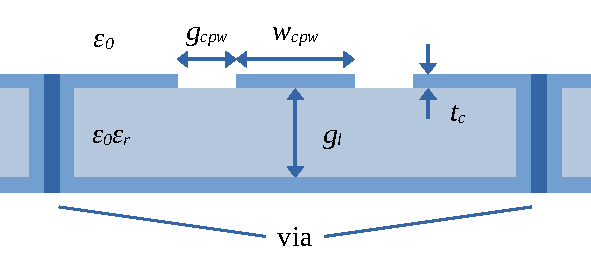
\includegraphics[width=0.6\textwidth]{kep/cpw.pdf}
	\caption{A rádió felől érkező koplanár tápvonal (CPW) keresztmetszete.}
	\label{fig:cpw}
\end{figure}
	A CPW tápvonal alapvetően jótulajdonságokkal rendelkezik. Csak kis mértékben diszperzív, mert a két vezető között az elektromos erővonalak nagy része az $\epsilon_r$ relatív dielektromos állandójú szubsztrátban záródik, így nincs nagy jelentőssége a levegőben és szubsztrátban terjedő rész-hullámok fázissebességbeli különbségének, egyszerűen QTEM közelítéssel kezelhető.
\section{Az antenna}
	Az antenna tervezésénél az első lépést az jelentette, hogy felderítsem a BIFA struktúrához tartozó, realizálható bemeneti impedancia tartományt, mert várhatóan a realizálható antenna bemeneti impedancia a fő korlátozó tényező a struktúra differenciális részének paraméterezésére nézve. Ezt a lépést egy relatíve egyszerű struktúrával végeztem, aminek a különböző méretparamétereinek hangolásával értem el a különböző valós bemeneti impedanciákat a bemeneten. Ez a struktúra \aref{fig:egyszeru.bifa}. ábrán látható.
\par A lépés lényegében próbálkozásból állt, különböző rögzített paraméterek mellett hangoltam ki az antennát a kérdéses sávon valós impedanciára.